\documentclass{article}
\usepackage[utf8]{inputenc}
\usepackage{amsmath,amssymb,amsbsy}
\usepackage{graphicx}
\usepackage[letterpaper,lmargin=2.0cm,rmargin=2.0cm,tmargin=2.0cm,bmargin=2.0cm]{geometry}
\usepackage{color}
\usepackage{listings}
\usepackage{indentfirst}
\usepackage{multirow}
\usepackage{listings}
\usepackage[round]{natbib} 
\usepackage{listings-python-options}
\usepackage{float}

\usepackage{hyperref}
\usepackage{url}
\title{Analysis Of Perceptron Algorithm And Its Variants Using Predefined Datasets}
\author{Harshil Shah\\Computer Science\\Colorado State University}
\date{September 14, 2015}

\begin{document}
\maketitle

\noindent
\hrulefill
\vspace{-5mm} 
\tableofcontents
\noindent
\hrulefill
\setlength{\parindent}{5ex} 

\section{Introduction}
Component of learning, in machine learning, is to divide the data according to its characteristics using machine learning techniques. [ ~\citep{Online1} ]Algorithms will be trained using predefined training data set and using classification results, trained algorithm will be applied on test data set. Simplest learning model suggests that data may satisfy the predefined hypothesis or they may not (binary). Best way to classify the data, will be to draw a line which will divide data set into two parts. Simplest algorithm for obtaining the satisfactory results, will be \textbf{Perceptron Learning Algorithm(PLA)}. So many variants were also proposed on PLA and are discussed in this document. The learning paradigm that is discussed, till now, is called  \textbf{Supervised Learning}. When the training data contains explicit examples of what the correct output should be for given inputs, then type of learning is called Supervised Learning. As far as this document is concerned, \textit{Supervised Learning} technique will be used only. [ \cite{Book1} ]
\subsection{Proposed Approach}
I have applied 4 machine learning algorithms - PLA without bias, PLA with bias, Pocket algorithm, Modified Perceptron algorithm - on 2 data sets - Heart Disease Data Set and Gisette Data Set, and analysis of result is provided. Furthermore, I have created learning curve depicting classifier accuracy as a function of the number of training examples, with the use of observation generated by applying PLA with bias on Gisette data set. Effects of normalization(Scaling and Standardization) on data set are also analyzed. 
\section{Perceptron Algorithm \& Its Variants}
Simplest algorithm of linear classifier is the perceptron algorithm. It is an algorithm for supervised learning of binary classifiers. In the nutshell, it is used for a function which maps input \(x\)(vector) to an output value
\(f(x)\) (binary).[ ~\citep{Online1} ]
\begin{equation}
f(x) = 
\begin{cases} 
1 & : \text{if  } w \cdot x + b > 0 \\
0 & : \text{otherwise}
\end{cases}
\end{equation}
where \(w\) is the weight vector, \(w \cdot x\) is dot product. \(\sum_{i=1}^{d} w_ix_i\), where \(m\) is number of features in dataset and \(b\) is the bias.\\
\par Formula can be more compactly written as [ \cite{Book1} ] 

\begin{equation}
f(x) = sign((\sum_{i=1}^{d} w_ix_i) + b)
\end{equation}
\par The perceptron learning algorithm will not terminate if the data set is not linearly separable. It will fail to reach the result where all data points will be properly classified.
\par Within the infinite space of all weight vectors , the perceptron algorithm will find a weight vector that works, using a simple iterative process. Upcoming sections will throw insights on how algorithm will work.

\subsection{Implementation of Variants}
\subsubsection{Classic Perceptron Algorithm (Without Bias)}
Simplest form of PLA is without using bias term. PLA will find \(w\) using a simple iterative method. At iteration \(t\), where \(t\) = 0 , 1, 2, . . . , there is a current value of the weight vector - \(w(t)\) . The algorithm picks an data from the data set that is currently misclassified, uses it to update \(w(t)\). The update rule is[ \cite{Book1} ]
\begin{equation}
w(t + 1) = w(t) + y (t)x(t)
\end{equation}
\par As equation suggests, final classifier will pass through origin and will always be dependant on product of input data and corresponding output sign.
\par Code snippet regarding this algorithm is shown as below.

\begin{lstlisting}
self.w = np.zeros(len(X[0]))
#initializing w to zero
    converged = False
    iterations = 0
    while (not converged and iterations < self.max_iterations) :
        converged = True
        for i in range(len(X)) :
            if y[i] * self.discriminant(X[i]) <= 0 :
                self.w = self.w + y[i] * self.learning_rate * X[i]
                converged = False
        iterations += 1
\end{lstlisting}
\subsubsection{Perceptron Algorithm With Bias}
PLA with bias works the same as PLA without bias. The bias shifts the decision boundary away from the origin and is independent of any input value.
\par As far as python code is concerned, only small alternation was needed. While retrieving data from data set, code will append one more element to feature set of each row, with having value of '1'. So produced \(w's\) first element will be bias for classifier. 
\begin{equation}
X_i,_0 = 1
\end{equation}
\par Code snippet regarding this algorithm is shown as below.
\begin{lstlisting}
#X will have one more element that will be appended on starting of array for each row.
#So that X[0] = 1 & self.w[0] = w0 after first iteration
self.w = np.zeros(len(X[0]))
#initializing w to zero
    converged = False
    iterations = 0
    while (not converged and iterations < self.max_iterations) :
        converged = True
        for i in range(len(X)) :
            if y[i] * self.discriminant(X[i]) <= 0 :
                self.w = self.w + y[i] * self.learning_rate * X[i]
                converged = False
        iterations += 1
\end{lstlisting}
\subsubsection{Pocket Algorithm}
The pocket algorithm solves the stability problem of original perceptron learning by keeping track of the best solution observed so far "in its pocket"(in memory). At the end, the best observed weight vector will be returned as the final classifier. The original PLA only checks some of the examples using \(w(t)\) to identify misclassification in each iteration, while the pocket algorithm needs an additional computation that evaluates all examples using \(w(t+1)\) to get \(E_{in}(w(t+1))\) . The additional computation makes the pocket algorithm much slower than original PLA.[ \cite{Book1} ] [ ~\citep{Online1} ]
\par The pocket algorithm can be also used for non-separable data sets, where the goal is to find a perceptron with a small number of misclassifications. However, the pocket algorithm does not guarantee the solution to show up within a given number of learning steps.[ \cite{Book1} ] [ ~\citep{Online1} ]
\par Code snippet regarding this algorithm is shown as below.

\begin{lstlisting}
self.wPocket = np.zeros(len(X[0]))
misClassifiedTracker = 0
misClassifiedPocketTracker = len(X)
converged = False
iterations = 0
while (not converged and iterations < self.max_iterations) :
    converged = True
    for i in range(len(X)) :
        if y[i] * self.discriminant(X[i]) <= 0 :
            self.w = self.w + y[i] * self.learning_rate * X[i]                    
            converged = False
    iterations += 1  
    misClassifiedTracker = 0
    for j in range(len(X) :
        if y[j] * self.discriminant(X[j]) <= 0 :
            misClassifiedTracker += 1
    if misClassifiedTracker < misClassifiedPocketTracker :
        misClassifiedPocketTracker = misClassifiedTracker
        self.wPocket = np.copy(self.w)

    self.w = self.wPocket
    self.converged = converged
\end{lstlisting}
\subsubsection{Modified Perceptron Algorithm}
The Modified Perceptron Algorithm works on a very simple principle - \textit{'One Problem At A Time'}. Principle suggests that, if error is encountered, then try to solve that error only with, of course, best possible solution, instead of considering other error's influence. \par According to algorithm, if mis-classified point is encountered, algorithm will try to find best solution by scanning whole dataset again. It may be possible that solution may not make mis-classified point classified, but it will still update weight vector \(w\). Algorithm will terminate if it has completely converged or maximum number of iteration has passed. 
\par Unlike other algorithms, Mis classification of data is decided based on  \(\lambda\) and product of some constant(\(c\)) variable and norm of weigh vector (\(w\)). If \(\lambda\) of \(i\) is less, then the product of \(c\) and norm of \(w\) then data is said to mis classified. Algorithm then find best weight vector using training dataset, that will help \(\lambda\) to get maximized. The key idea behind such condition for mis classification is to converge the points which are nearby the weight vector first.
\par Code snippet regarding this algorithm is shown as below.
\begin{lstlisting}
self.w = np.random.uniform(-1, 1, len(X[0]))
#Initializing w to random lowest values
#Initializing Constant C to 0.01 too.
converged = False
iterations = 0
needToChangeW = True
while (not converged and iterations < self.max_iterations) :
    converged = True
    needToChangeW = False
    for i in range(len(X)) :
        neededI = 0
        maxLembda = y[i] * self.discriminant(X[i])
        if y[i] * self.discriminant(X[i]) < self.constantC * np.sqrt(np.dot(self.w, self.w)) :
            for j in range(len(X)) :
                tempW = self.w + y[j] * self.learning_rate * X[j]
                tempLambda = y[i] * np.dot(tempW, X[i])
        
                if maxLembda < tempLambda :
                    maxLembda = tempLambda
                    neededI = j
            self.w = self.w + y[neededI] * self.learning_rate * X[neededI]
            needToChangeW = True
            converged = False

    if(not needToChangeW) :
        converged = True
    else :
        converged = False
    iterations += 1
    self.converged = converged
        
\end{lstlisting}
\subsection{Analysis of Results}
Training and testing datasets for provided datasets - Heart Disease Dataset and Gisette Dataset - are created randomly for sake of analyzing algorithms. Heart Disease training dataset contains 170 data entries, whereas Gisette training dataset contains 4500 data entries. PLA and its variants' implementation is explained earlier. All algorithms are applied on two randomly generated datasets.
\par Observations are noted by applying all algorithms to both datasets by changing maximum number of iterations of algorithm and algorithms' learning rate. For each observation \(E_{in}\) and \(E_{out}\) are also calculated. The out-of-sample error \(E_{out}\) measures how well training on N examples has generalized to data that have not been seen before. Whereas, the in-sample error \(E_{in}\)  , by contrast , is based on data points that have been used for training. Below shown two formulas are used to calculate in-sample and out-of-sample error.[ \cite{Book1} ]
\begin{equation} 
E_{in} = \cfrac{\text{Number of Misclassification in Training Dataset Found Using Converged \(w\)}}{\text{Total Number of Example in Training Dataset}}\\
\end{equation}
\begin{equation} 
E_{out} = \cfrac{\text{Number of Misclassification in Test Dataset Using Converged \(w\) Found Using Training Dataset}}{\text{Total Number of Example in Test Dataset}}\\
\end{equation}
\begin{table}[H]

\begin{center}
\begin{tabular}{ |c|c|c|c|c| } 
\hline
\multicolumn{5}{|c|}{Heart Disease Data Set} \\
\hline
\hline
Algorithm Applied & Iteration Used & Learning Rate & \(E_{in}\) & \(E_{out}\) \\
\hline
\hline
\multirow{3}{5em}{Perceptron Without Bias} & 100 & 0.3 & 0.247058823529 & 0.3 \\ 
& 200 & 0.5 & 0.241176470588 & 0.3 \\ 
& 400 & 0.3 & 0.229411764706 & 0.27 \\ 
\hline
\hline
\multirow{4}{5em}{Perceptron With Bias} & 100 & 0.3 & 0.247058823529 & 0.3 \\ 
& 200 & 0.3 & 0.241176470588 & 0.3 \\ 
& 200 & 0.5 & 0.241176470588 & 0.3 \\ 
& 400 & 0.3 & 0.229411764706 & 0.26 \\ 
\hline
\hline
\multirow{4}{5em}{Pocket Algorithm} & 100 & 0.3 & 0.241176470588 & 0.34 \\ 
& 200 & 0.3 & 0.205882352941 & 0.27 \\ 
& 200 & 0.5 & 0.205882352941 & 0.27 \\ 
& 400 & 0.3 & 0.176470588235 & 0.27 \\ 
\hline
\hline
\multirow{5}{5em}{Modified Perceptron (C = 0.01)} & 50 & 0.3 & 0.388235294118 & 0.36 \\ 
& 100 & 0.3 & 0.405882352941 & 0.35 \\ 
& 200 & 0.3 & 0.417647058824 & 0.35 \\ 
& 200 & 0.5 & 0.417647058824 & 0.35 \\ 
& 400 & 0.3 & 0.429411764706 & 0.35 \\ 
\hline


\end{tabular}
\caption{Results Produced When Algorithms Applied On Heart Disease Data Set}
\end{center}
\end{table}
\par All algorithms are applied on heart disease dataset and according to data observed, it can be said that, heart disease dataset is not linearly converging by any of the algorithm. As far as accuracy is concerned, all algorithm, except modified algorithm, seems to be producing almost same results. Increasing learning rate is not affecting any of the algorithm. Furthermore, increasing number of iteration is not widely affecting either of PLA without bias term and with bias term. Though, pocket algorithm becomes more powerful with the increase of number of iteration. Reason for becoming more efficient with increasing iteration is, algorithm keeps its best solution in its pocket. Worst algorithm, out of four, is modified algorithm. With the increase of number of iteration or increase in learning rate or increase in constant \(C\), algorithm is not tending towards solution line. After having 400 iterations, modified algorithm is converged only nearly 58\% which is almost 25\% lesser than pocket algorithm. Out of 4 algorithms - PLA and its variant - pocket algorithm seems to be more accurate.  
\begin{table}[H]
\begin{center}
\begin{tabular}{ |c|c|c|c|c| } 
\hline
\multicolumn{5}{|c|}{Gisette Data Set} \\
\hline
\hline
Algorithm Applied & Iteration Used & Learning Rate & \(E_{in}\) & \(E_{out}\) \\
\hline
\hline
{Perceptron Without Bias} & 14 & 0.1 & 0.0 & 0.0353333333333 \\ 

\hline
\hline
Perceptron With Bias & 14 & 0.1 & 0.0 & 0.0353333333333 \\
\hline
\hline
Pocket Algorithm & 14 & 0.1 & 0.0 & 0.0353333333333 \\
\hline
\hline
Modified Perceptron (C = 0.01) & 10 & 0.2 & 0.0 & 0.0293333333333 \\
\hline
\hline
Modified Perceptron (C = 0.05) & 14 & 0.2 & 0.0 & 0.0353333333333 \\
\hline
\hline
Modified Perceptron (C = 0.001) & 14 & 0.2 & 0.0 & 0.0353333333333 \\
\hline
\end{tabular}
\caption{Results Produced When Algorithm Applied On Gisette Data Set}
\end{center}
\end{table}
PLA and its all variants are also applied on Gisette dataset, and as shown in table, all algorithms are converging on dataset. It means that, given Gisette dataset is linearly separable. All algorithms are producing almost same results and are getting converged in 14 iterations with having \(E_{out}\) of 0.035 only. As weight vector(\(w\))  is getting initialized to random value in modified perceptron algorithm, it changes the frequency of getting converged. 
For all other algorithms, weight vector (\(w\))  is getting initialized to array of zeros for both datasets.
\par Learning Curves for all algorithms is generated. (consider fig(\ref{1 Learning Curve}) and fig(\ref{1.1 Learning Curve})). Number of maximum iteration that can be used is set to 50, learning rate is set to 0.2 and constant \(C\) is set to 0.01. For both datasets, learning curves for all algorithm is shown below.

\begin{figure}[H]
  \centering
    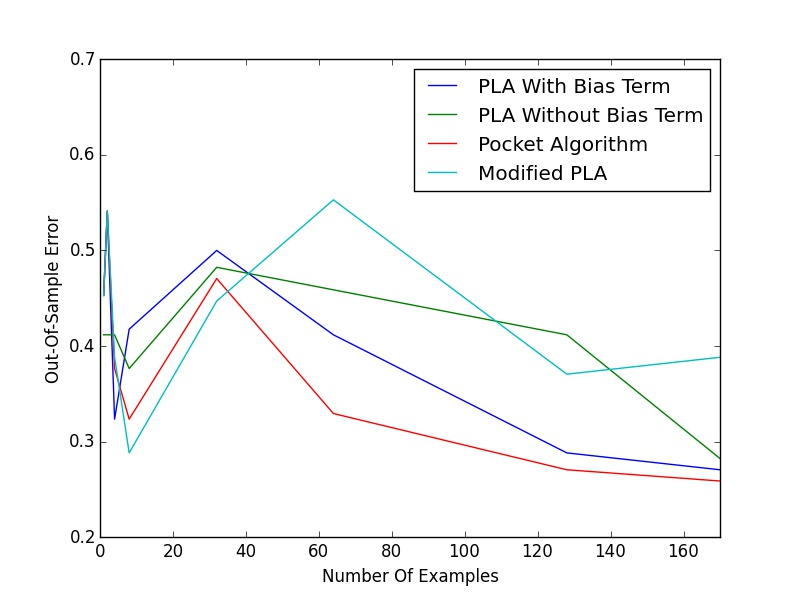
\includegraphics[width=6in]{images/LCOfAll_Heart_Data.jpeg}
   
    \caption{Learning Curve Generated By Applying All Perceptron Algorithm On Heart Disease Data }
    
    \label{1 Learning Curve}
  
\end{figure}
\par To draw learning curve for heart disease dataset, number of examples used for training algorithm is in logarithmic scale - 1, 2, 4, 8, 16, 32, 64, 128, 170. Above shown figure depicts learning curves for heart disease dataset. As discussed earlier and figure (\ref{1 Learning Curve}) also agrees that pocket algorithm is more efficient than any others \& modified PLA is giving worst performance. 
\begin{figure}[H]
  \centering
    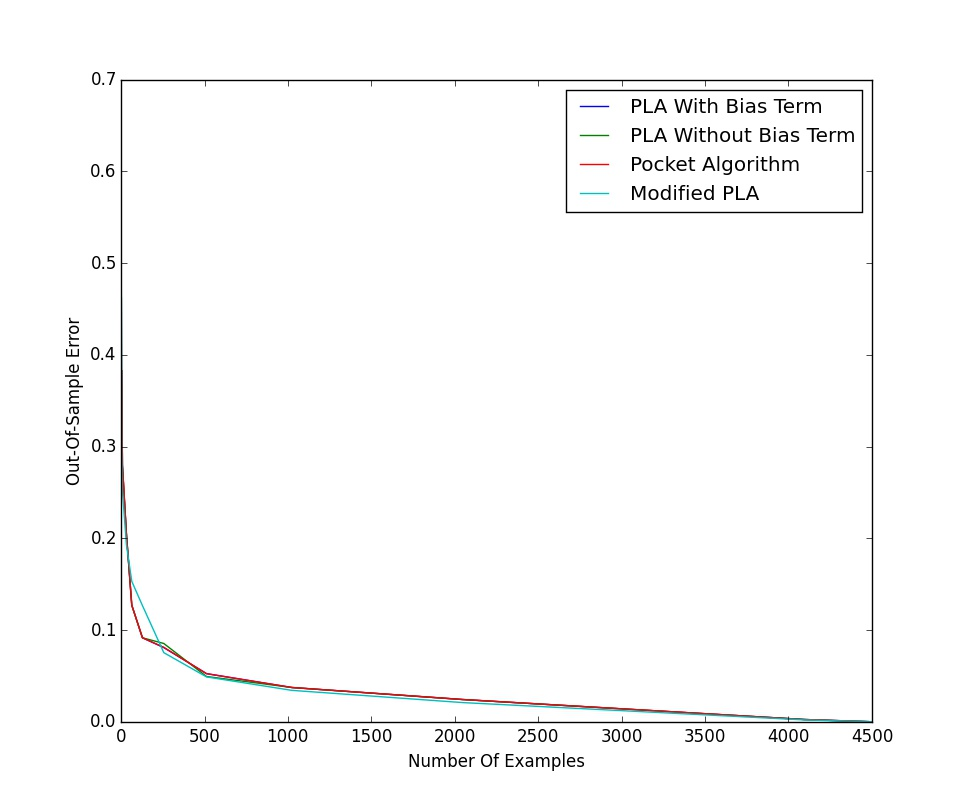
\includegraphics[width=6in]{images/LCOfAll_Gisette_Data.jpeg}
   
    \caption{Learning Curve Generated By Applying All Perceptron Algorithm On Gisette Data }
    
    \label{1.1 Learning Curve}
  
\end{figure}
To draw learning curve for Gisette dataset, number of examples used for training algorithm is in logarithmic scale - 1, 2, 4, 8, 16, 32, 64, 128, 256, 512, 1024, 2048, 4096, 4500. Above shown figure depicts learning curves for Gisette dataset. All algorithms converge with almost same accuracy. Graph also depicts that, with the increase of number of examples, algorithms' accuracy is increasing. Graph also depicts minimum number of examples required to get full convergence. 
\section{Learning Curves}
Learning Curve represent the generalization performance of the model, i.e. accuracy  of the learning system as a function of the size of the training set. It  can give an abstract view of how many training examples will actually be needed to converge the dataset. Graph can be very useful for predicting whether given dataset is actually linearly separable or not. Furthermore, curve can also depict how many examples of dataset will actually be needed to get algorithm start to learn. Given dataset is said to be fully converged with the use of linear model if curve tends to zero error line . After adding few example, curve will become constant, which depicts the best achievable accuracy of the given model. [ \cite{Book1} ]



\begin{figure}[H]
  \centering
    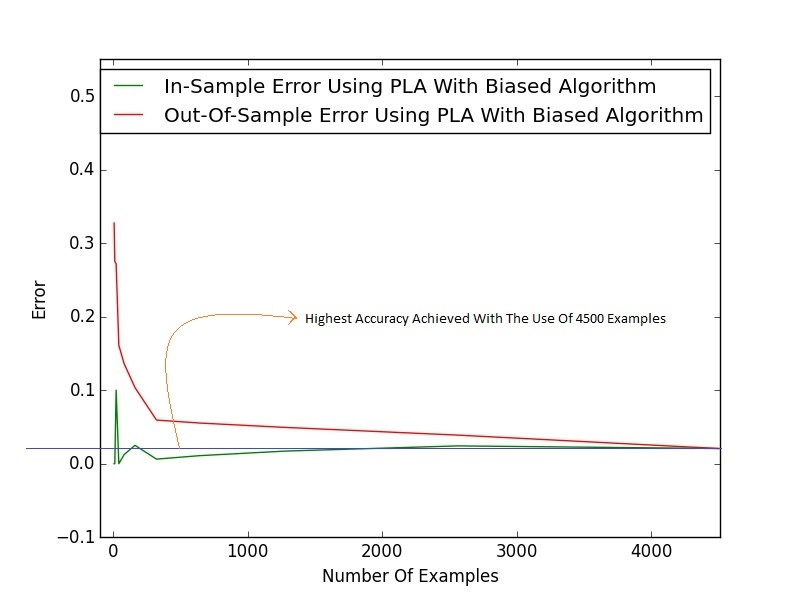
\includegraphics[width=6in]{images/LC.jpeg}
    \caption{Learning Curve Generated By Applying Perceptron Algorithm With Bias On Gisette Dataset}
    \label{2. Learning Curve}
  
\end{figure}
\par Above graph illustrates the learning curves for a simple learning model - PLA with bias term - based on actual experiments with the use of Gisette dataset. Number of examples used are in logarithmic scale - 5, 10, 20, 40, 80, 160, 320, 640, 1280, 2560, 4500. Notice that for the model, the learning curves converge quickly. This behavior is typical in practice. With the increase of learning examples, the out-of-sample learning curve is decreasing , while the in-sample learning curve is increasing. As it is easily observable that, learning curve is tending towards zero error line. Right now, as graph suggest, accuracy of algorithm is in order of 0.01. If it possible to add more training dataset, then algorithm may end up converging dataset. Illustrated learning curves are the perfect example of such models which are to converge training example, but may fail to converge testing dataset. 
\section{Data Normalization}
Feature scaling is a method used to normalize the range of independent variables or features of data. In machine learning, it is also known as data normalization and is generally performed during the data pre-processing step. In machine learning, the most of the machine learning algorithms, classifiers calculate the distance between two points by the euclidean distance. If one of the features has a wide range of values, the distance will be decided by this particular feature only.  Since the range of values of data varies widely, machine learning algorithms will not work properly without normalization. Furthermore, steepest descent (gradient descent) converges much faster with feature scaling than without it. Report contains two basic types of normalization - \(Scaling\) \textit{(also called Rescaling)} and \(Standardization\) [ ~\citep{Online2} ]
\subsection{Scaling}
The simplest form of normalization is scaling. Objective of this report is to scale data in the range of -1 to +1. Selecting the target range depends on the nature of the data. \\
\par The general formula is given as:[ ~\citep{Online3} ]
\begin{equation} 
X_{i,a to b} = \cfrac{(b - a) (X_i - X_{max)}}{X_{max} - X_{min}} + a
\end{equation}
Where:\\
\(X_i\) = Each data point\\
\(X_{min}\) = Minimum value for feature\\
\(X_{max}\) = Maximum value for feature\\
\(X_{i,a to b}\) = Data point \(i\) normalized between \(a\) and \(b\)\\
\par As far as this report is concerned, scaling will be done in range of -1 to 1. So formula used for scaling is as below:
\begin{equation} 
X_{i,-1 to 1} = \cfrac{2 * (X_i - X_{max)}}{X_{max} - X_{min}} - 1
\end{equation}
\par Code snippet regarding this logic is shown as below.
\begin{lstlisting}
#X hold original dataset features
#X is ndarray
maxValue = X.max(axis=0)
minValue = X.min(axis=0)
for i in range(len(X)) :
    innerScaleArray = [1]
    for j in range(len(X[0])-1) :
        difference = (maxValue[j+1] - minValue[j+1])
        innerScaleArray.append((((inputArray[i][j+1] - minValue[j+1]) / difference)*2) - 1)
        #Scaling Logic
    inputArrayScaled.append(innerScaleArray)
    
X_scaled = np.asarray(inputArrayScaled)
\end{lstlisting}
\subsubsection{Analysis of Scaling}
Heart Disease dataset has been scaled to range of -1 to 1. The Perceptron with bias term linear algorithm was applied on the scaled version dataset and original dataset, and below observation was captured with different iterations. Furthermore, learning curves were drawn for both scaled and original datasets (consider fig(\ref{2.5 Learning Curve}) and fig(\ref{3. Learning Curve})). 

\begin{table}[H]
\begin{center}
\begin{tabular}{ |c|c|c|c| } 
\hline
\multicolumn{4}{|c|}{Heart Disease Data Set} \\
\hline
\hline
Iteration Used & Learning Rate & \(E_{out}\) \textit{(Using Original Dataset)} & \(E_{out}\) \textit{(Using Scaled Dataset)} \\
\hline
\hline
1 & 0.2 & 0.49411764705882355 & 0.17058823529411765 \\ 

\hline
\hline
10 & 0.2 & 0.38235294117647056 & 0.18235294117647058 \\
\hline
\hline
40 & 0.2 & 0.2823529411764706 & 0.1411764705882353 \\


\hline
\hline
60 & 0.2 & 0.27058823529411763 & 0.17058823529411765 \\


\hline
\hline
100 & 0.2 & 0.25882352941176473 & 0.12941176470588237 \\

\hline
\end{tabular}
\caption{Effect of Scaling on Dataset}
\end{center}
\end{table}
\par Above table was generated by changing value of number of iterations to see efficiency and speed of converging by applying same algorithm on both datasets. After first iteration of algorithm on original dataset, still nearly 50\% of data remained not converged. While, after first iteration of algorithm on scaled version of original dataset, nearly 17\% of data remained not converged. Furthermore, algorithm could not reach the same efficiency in 100 iterations using original dataset as it achieved in only 1 iteration on scale version. To know reason, consider below table.  
\par Table is generated based on number occurrence of feature in specific range in original unscaled version and scaled version. \textit{(Training dataset was randomly selected containing 170 example entries.)}
\begin{table}[H]
\begin{center}
\begin{tabular}{ |c|c| } 
\hline
\multicolumn{2}{|c|}{Heart Disease Data Set } \\
\hline
Range & Number of Features\\
\hline
\hline
400-500 & 1\\
\hline
\hline
300-400 & 23\\
\hline
\hline
200-300 & 122\\
\hline
\hline
100-200 & 352\\
\hline
\hline
0-100 & 1707\\
\hline
\end{tabular}
\begin{tabular}{ |c|c| } 
\hline
\multicolumn{2}{|c|}{Heart Disease Scaled Data Set } \\
\hline
Range & Number of Features\\
\hline
\hline
0.6 to 1 & 488\\
\hline
\hline
0.2 to 0.6 & 264\\
\hline
\hline
-0.2 to 0.2 & 310\\
\hline
\hline
-0.6 to -0.2 & 297\\
\hline
\hline
-1 to -0.6 & 851\\
\hline
\end{tabular}
\caption{Comparison Of Feature Occurrence In Specific Range In Original And Scaled Dataset}
\end{center}
\end{table}
\par PLA with bias term tries to reach the classifier by calculating euclidean distance between two points. Now according to table shown above, distance between two example in original version will be fairly very large as most of the points are in range 0-100. We need to take account of all points and as distance is huge, algorithm might take more iterations to reach the needed answer. Now, after scaling, data points are fairly distributed all across the range from -1 to 1. Thus, within only 1st iteration, algorithm can converge more number of points than converging on unscaled version.
\par Learning Curves, to understand effectiveness of scaling, can be also drawn. Below graph depicts the learning curves showing efficiency of using scaled version of original dataset. 40 iterations are used on number of training example and out-of-sample errors are calculated. Number of training examples are in logarithmic scale - 1, 2, 4, 8, 16, 32, 64, 128.
\begin{figure}[H]
\centering
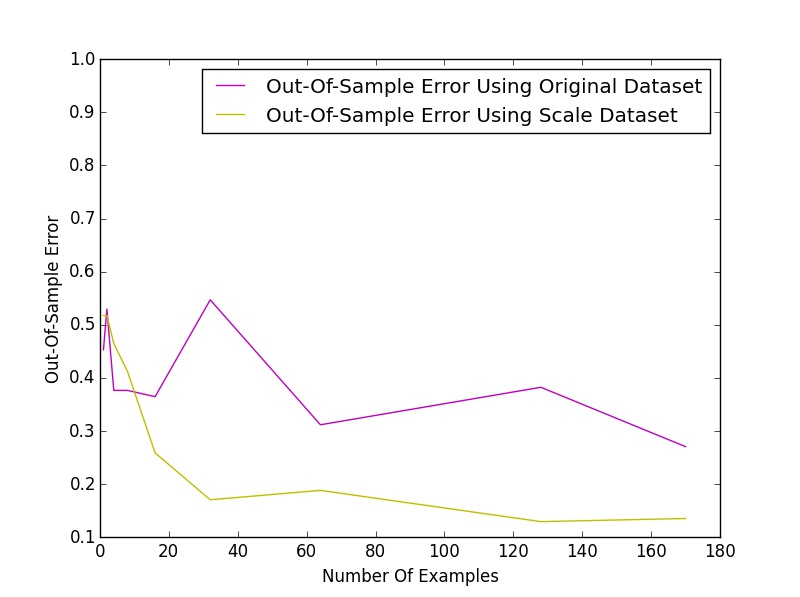
\includegraphics[width=5in]{images/40Iter_Normalized.jpeg}
\caption{Learning Curve Based On Original Dataset, Scaled Dataset Using 40 Iterations}
\label{2.5 Learning Curve}
  
\end{figure}
\par Clearly, it is observable from the figure that scaled version of dataset is getting converged faster and with higher accuracy too. Now, instead of using only logarithmic number of example, below graph is created using all possible range of number of example.
\begin{figure}[H]
\centering
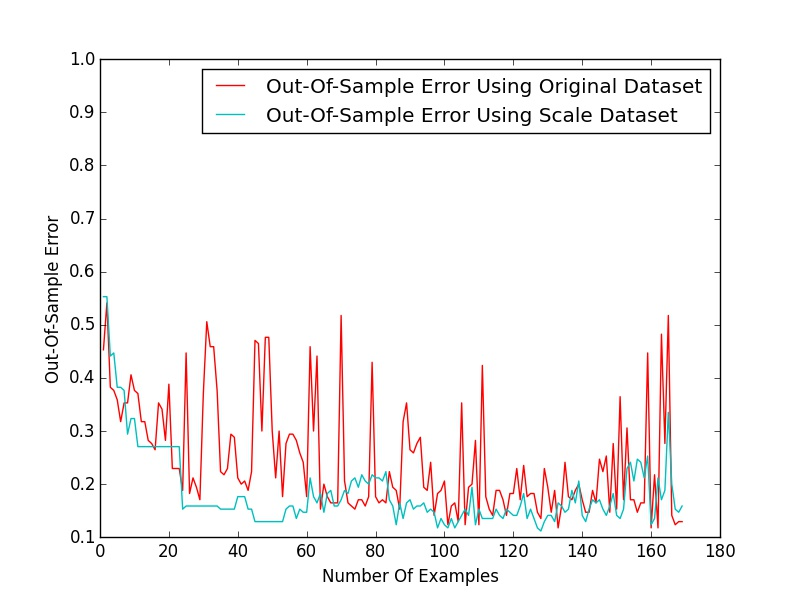
\includegraphics[width=6in]{images/LearningCurveForNormalizationVsOriginal.jpeg}
\caption{Learning Curve Based On Original Dataset, Scaled Dataset Using All Possible Examples}
\label{3. Learning Curve}
  
\end{figure}
\par Above drawn graph depicts that frequency of change of out-of-sample errors with the increase of number of example is low if algorithm is applied on scaled version of dataset.
\subsection{Standardization}
In machine learning, data can include multiple dimensions(features). Feature standardization makes the values of each feature in the data have zero-mean and a unit-variance. 
[ ~\citep{Online3} ]
\begin{equation} \label{eq:3}
\bar{X_{i}} = \cfrac{X_i - X_{i, mean}}{ \sigma_i}
\end{equation}
Where:\\
\(\bar{X_{i}}\) = Standardized data point\\
\(X_i\) = Each data point\\
\(X_{i, mean}\) = Mean of \(X_i\)\\
\(\sigma_i\) = Standard Deviation \\



\par Dividing each value by the standard deviation, generates transformed variables with variances of 1 (unit variance), but different means and ranges and hence standardized version will be as meaningful as original dataset. Range(i.e. maxValue - minValue) in standardized data gives idea about the distribution of the data with respect to mean line.

\par Code snippet regarding this logic is shown as below.
\begin{lstlisting}
#X hold original dataset features
#X is ndarray
maxValue = X.max(axis=0)
minValue = X.min(axis=0)
    
standardD = np.std(X, axis=0)
standardD[0] = 1
meanArrays = X.mean(axis=0) 
meanArrays[0] = 0
X_Standardized = (X - meanArrays) / standardD
\end{lstlisting}
\subsubsection{Analysis of Standardization}
Heart Disease dataset has been standardized using above mentioned formula( see formula(\ref{eq:3})). The Perceptron with bias term linear algorithm was applied on the standardized version dataset and scale dataset, and below observation was captured with different iterations. Furthermore, learning curves were drawn for both scaled and standardized datasets.(consider fig(\ref{4. Learning Curve}) and fig(\ref{5. Learning Curve}))
\begin{table}[H]
\begin{center}
\begin{tabular}{ |c|c|c|c| } 
\hline
\multicolumn{4}{|c|}{Heart Disease Data Set} \\
\hline
\hline
Iteration Used & Learning Rate & \(E_{out}\)\textit{(Using Scaled Dataset)} & \(E_{out}\)\textit{(Using Standardized Dataset)} \\
\hline
\hline
1 & 0.2 & 0.1588235294117647 & 0.18235294117647058 \\ 

\hline
\hline
10 & 0.2 & 0.17647058823529413 & 0.19411764705882353 \\
\hline
\hline
40 & 0.2 & 0.17058823529411765 & 0.17647058823529413 \\


\hline
\hline
60 & 0.2 & 0.17058823529411765 & 0.18823529411764706 \\


\hline
\hline
100 & 0.2 & 0.15294117647058825 & 0.20588235294117646 \\

\hline
\hline
150 & 0.2 & 0.16470588235294117 & 0.20588235294117646 \\
\hline
\end{tabular}
\caption{Effect Of Standardization On Dataset}
\end{center}
\end{table}
\par Above table was generated by changing value of number of iterations to compare efficiency and speed of converging by applying same algorithm on both datasets. Algorithm seems to be working with almost the same accuracy on both dataset. But, still, with minor difference of nearly 2-3\%, scaled data seems to get converged more accurately.\\

\par Learning curves depicting accuracy of scaling and standardization, can be also drawn. To generate below shown learning curves, 60 iterations of algorithm are used on number of training example and out-of-sample errors are calculated. Number of training examples used are in logarithmic scale - 1, 2, 4, 8, 16, 32, 64, 128
\begin{figure}[H]
\centering
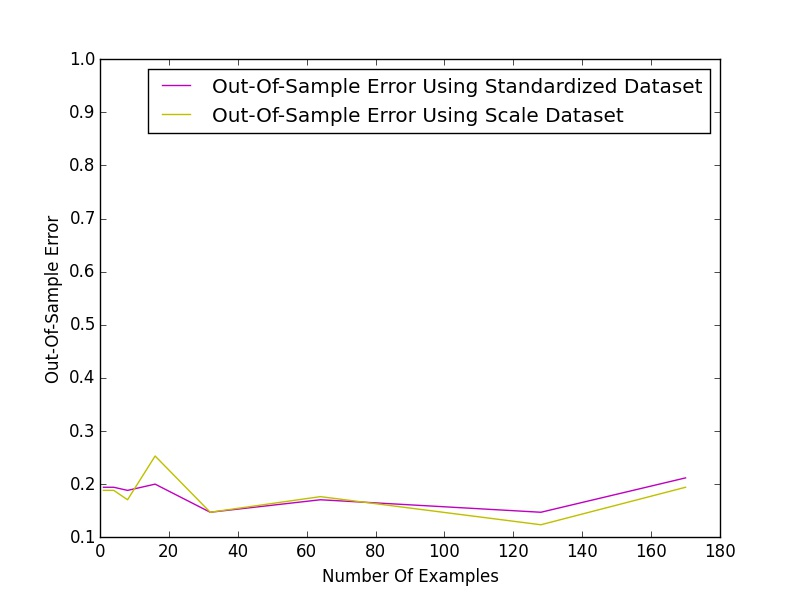
\includegraphics[width=5in]{images/60Iter_Standardized.jpeg}
\caption{Learning Curve Based On Scaled Dataset, Standardized Dataset Using 60 Iterations}
\label{4. Learning Curve}
  
\end{figure}
\par As seen in above figure, algorithm seems to be working with almost same accuracy and same notion on both scaled and standardized data. Now, instead of using only logarithmic number of example, below graph is created using all possible range of number of example to get proper idea about frequency of change in nature of algorithm with respect of increase of number of training example.
\begin{figure}[H]
\centering
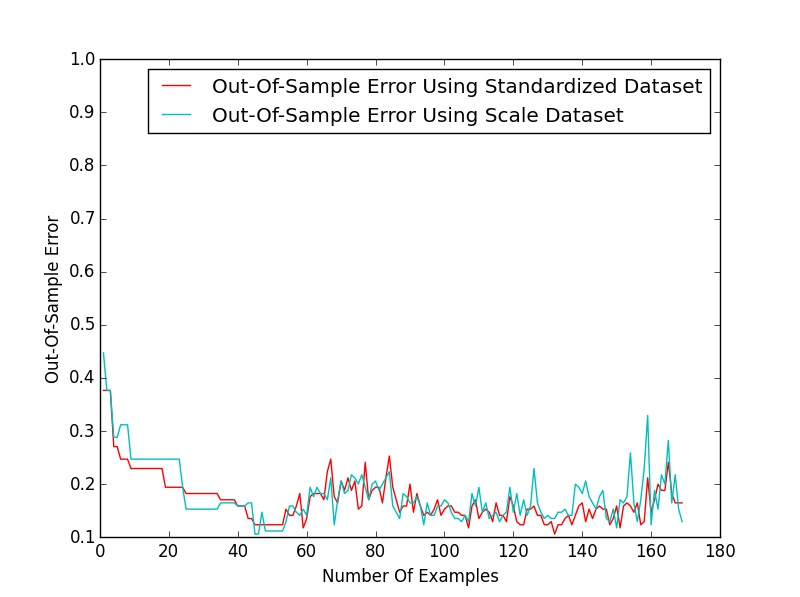
\includegraphics[width=5in]{images/LearningCurveForStandardizedVSNormalization.jpeg}
\caption{Learning Curve Based On Scaled Dataset, Standardized Dataset Using All Possible Examples}
\label{5. Learning Curve}
  
\end{figure}
\par According to above shown figure, nature of algorithm on both dataset remains almost same. Still, algorithm's nature flickers more when applied on scaled version than standard version. Characteristic of standardization - keeping relative information of data plots - explains the less flickering on changing of number of training examples. 

\par In the nutshell, standardization on data can be useful when number of features are too many. Standardization can also be used for the estimation of outliers. Scaling may not preserve effect of outliers but standardization will keep the effect of outliers intact. 
\subsection{Conclusion on Normalization}
To sum up with normalization, consider below drawn figure showing accuracy of PLA with bias algorithm when applied on original, scaled and standardized dataset.\
\begin{figure}[H]
\centering
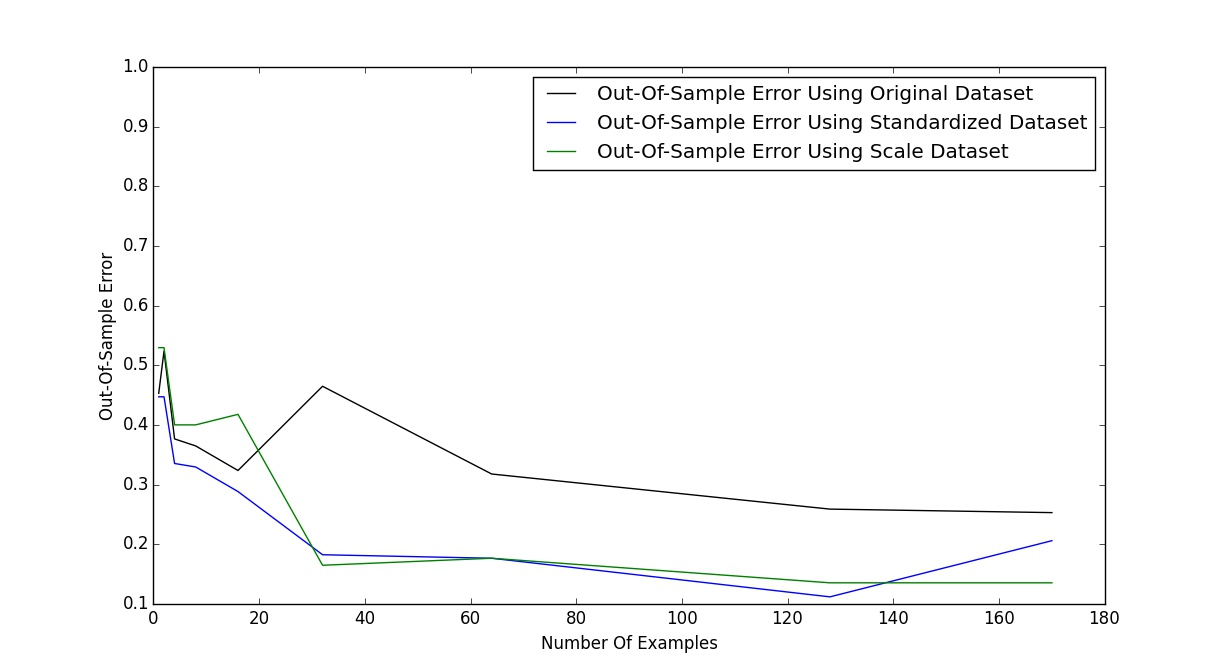
\includegraphics[width=6in]{images/Original_Norm_Stand.jpeg}
\caption{Learning Curve Based On Original, Scaled And Standardized Dataset}
\label{6. Learning Curve}
  
\end{figure}

\par 100 iterations were performed by an algorithm with having learning rate of 0.2 on all datasets and above shown learning curve was created. As far as accuracy and time to get converged is concerned, using the algorithm on scaled data seems more powerful and efficient.
\section{Conclusion}
\par To sum up, all algorithms have pros and cons. As far as this report is concerned, the pocket algorithm seems to be working more accurately than any other. Furthermore, instead of using algorithm on original dataset, if they are applied on normalized dataset, then they seemed to get converged faster and accurately. 
\bibliography{biblo.bib}
\bibliographystyle{plainnat}
\end{document}
